\documentclass[../main.tex]{subfiles}

\begin{document}

\section{Rigideces de elementos}

Cuando consideramos los conjuntos de desplazamientos horizontales $u$, 
verticales  $v$ y torsionales $\theta$, podemos encontrar el corrimiento
local de una subestructura como:


\begin{align*}
  u_p = - u * \sin{\phi * P} + v*\cos \phi*p + \theta * r_p
.\end{align*}

\begin{figure}[htpb]
  \centering
  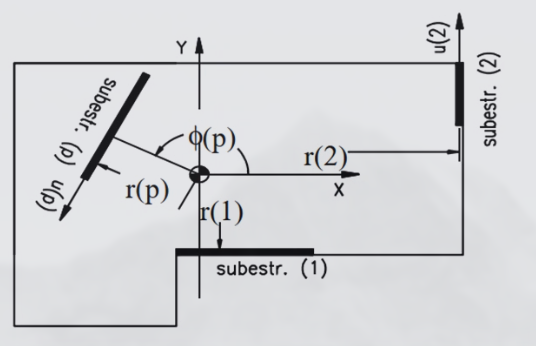
\includegraphics[width=0.8\textwidth]{../images/20210608/diagrama.png}
  \caption{Diagrama para ecuación}
  \label{fig:diagrama}
\end{figure}

\section{Tabiques de hormigón armado}

Se desarrollan en el capítulo 14 del CIRSOC 201. Los tabiques están normalmente
sometidos a carga axial, con o sin flexión, o pueden trabajar como muros de
corte.

La longitud total de un tabique $l_w$ que se considera efectiva cada carga
concentrada, debe ser:

 \begin{align*}
  l_w \leq \begin{cases} \text{ - que la distancia entre los centros de carga} \\
    \text{ - que el ancho del elemento o apoyo que transmite} \\
    \text{las cargas concentradas más cuatro veces el espesor del tabique}
  \end{cases}
.\end{align*}

Debemos tener en cuenta que este valor $l_w$ será distinto y menor al ancho
real de $d$, como se muestra en \Cref{fig:anchoefectivo}

\begin{figure}[htpb]
  \centering
  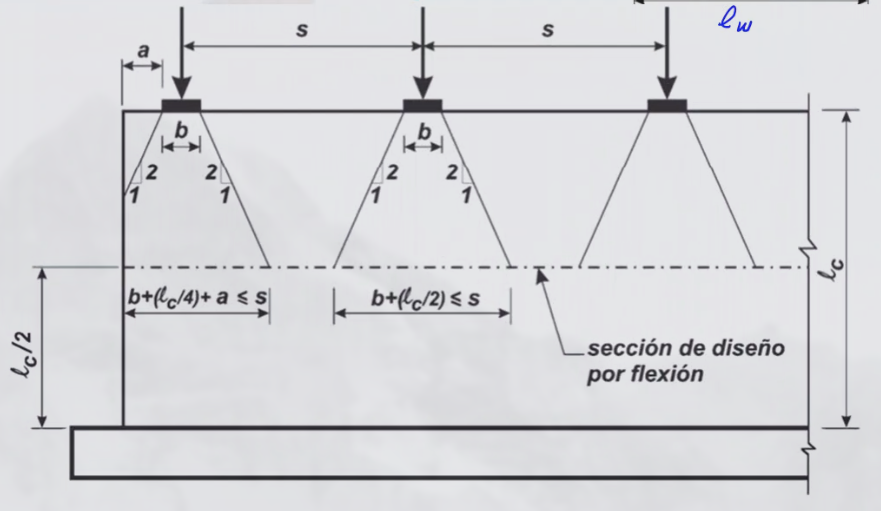
\includegraphics[width=0.8\textwidth]{../images/20210608/anchoefectivo}
  \caption{Ancho efectivo con cargas distribuidas.}
  \label{fig:anchoefectivo}
\end{figure}

Y donde el espesor del tabique, denominado $h$, será:

 \begin{align*}
  h \geq \begin{cases}
  \SI{10}{cm} \\
  min\left( \frac{l}{25};\frac{l_w}{25} \right) 
  \end{cases}
.\end{align*}

Donde el valor de $l$ es la altura de piso a techo de cada tramo.

\subsubsection{Armadura mínima}

La cuantía mínima de la armadura vertical referida a la sección completa
dependerá si es un muro que solo está sometido a esfuerzos axiales o se 
consideran esfuerzos de corte.

Se debe cumplir que $\rho_l$:

\begin{enumerate}
  \item \textbf{0.0012} para barras o alambre conformados por $d_b \leq 16mm$
    con $f_y\geq 420MPa$.
  \item \textbf{0.0015} para otras barras conformadas con $d_b\geq 16mm$.
  \item \textbf{0.0012} para mallas de acero soldadas de alambres lisos o
    conformados con $d_b \leq 16mm$.
\end{enumerate}

La cuantía mínima para la armadura horizontal referida a la sección total, se
debe cumplir que $\rho_t$:

\begin{enumerate}
  \item \textbf{0.002} para barras conformados con $d_b \leq 16mm$ y con
    $f_y \geq 420MPa$
  \item \textbf{0.0025} para otras barras conformadas con $d_b \geq 16mm$.
  \item \textbf{0.002} para mallas de acero.
\end{enumerate}

Además, siempre que se tenga un espesor mayor a 250mm de espesor, el mismo
es necesario que este armado en ambas caras.

En cuanto a la separación tendrá que ser:

\begin{enumerate}
  \item Igual o menor a tres veces el espesor del tabique.
  \item Igual o menor a 300mm.
\end{enumerate}

\subsubsection{Diseño empírico}

Si se toma el tabique bajo cargas gravitatorias y momentos que puede sea
alrededor de su eje débil (es decir, no trabando a corte), podemos utilizar
éste método.

Además se debe cumplir que:


\begin{itemize}
  \item La resultante de todas las cargas concentradas este ubicada en el tercio
  central del espesor total del tabique.
  \item Se satisfagan condiciones geométricas mínimas.
\end{itemize}

Entonces, la resistencia axial de diseño de un tabique, se puede determinar como
se ilustra en la expresión:

\begin{align*}
  \phi * P_n = 0.55 * \phi * f'_c * A_g * \left( 1 - \left( \frac{k*l_c}{32*h} \right)^{2}  \right) 
.\end{align*}

Donde podemos adoptar un valor de $k$, que es un factor de longitud efectiva,
dependiendo de si el tabique esta arriostrado contra el desplazamiento lateral o
no, de forma muy similar a como se hace en el pandeo, según la tabla del 
CIRSOC 201. Luego, las armaduras mínimas pueden ser obtenidas mediante 
diagramas de interacción  $M_u - P_u$.

\subsubsection{Dimensionamiento a corte}

Para la verificación al corte, se debe hacer un procedimiento muy similar al
procedimiento que se da en vigas. Primero, se considera una parte del valor
de $V_n$ como  $V_c$, que estará prefijado según las formulas del capítulo 11
del CIRSOC 201, particularmente, las expresiones \textbf{11.10.6}.

Luego, se debe verificar las expresiones  \textbf{11.29} y \textbf{11.30} para
obtener los valores de $V_c$ y verificar que se encuentre dentro de los
parámetros ya determinados.

En caso que se verifique la condición siguiente se podrá poner la armadura
mínima de corte, con una cuantía mínima de $\rho_t = 0.0025$.

 \begin{align*}
  V_n \leq  \phi * \frac{V_c}{2}
.\end{align*}


Donde la separación máxima deberá ser determinada.


\end{document}
